

\makesectionpage[figures/quiz.png]{Lineare Regression}

\begin{frame}{Lineare Regression}

\begin{columns}
\begin{column}{0.35\textwidth}

\textbf{Idee}: 
Wir legen eine lineare Funktion durch unsere Messwerte.

\vspace{0.8em}

Mit dieser Funktion können wir anschließend Werte
vorhersagen.

\[
\begin{aligned}
y            &= a \cdot x + b\\
\text{Miete} &= a \cdot \text{Größe} + b
\end{aligned}
\]

\end{column}


\begin{column}{0.6\textwidth}
\centering

\begin{tikzpicture}[
    x=0.045cm,
    y=0.0028cm,
    >=latex,
    font=\scriptsize,
    scale=1.2
]

    % Hintergrund
    \fill[BlockBackground] (0,0) rectangle (140,1600);

    % Horizontale Gitterlinien
    \foreach \yy in {200,400,...,1600}{
        \draw[DarkGrey!60, line width=0.4pt]
            (0,\yy) -- (140,\yy);
    }

    % Achsen
    \draw[TextColor, line width=1pt, ->] (0,0) -- (146,0);
    \draw[TextColor, line width=1pt, ->] (0,0) -- (0,1700);

    % x-Ticks
    \foreach \xx in {0,20,...,140}{
        \draw[TextColor] (\xx,0) -- (\xx,-35);
        \node[anchor=north,text=DarkGrey] at (\xx,-40) {\tiny \xx};
    }

    % y-Ticks
    \foreach \yy in {0,200,...,1600}{
        \draw[TextColor] (0,\yy) -- (-3,\yy);
        \node[anchor=east,text=DarkGrey] at (-4,\yy) {\tiny \yy};
    }

    % Achsenbeschriftungen
    \node[
        rotate=90,
        align=center,
        text=TextColor,
        font=\scriptsize\bfseries
    ] at (-19,800) {Monatsmiete in €};

    \node[
        align=center,
        text=TextColor,
        font=\scriptsize\bfseries
    ] at (70,-190) {Wohnungsgröße in qm};

 

    % Messpunkte
    \foreach \x/\y in {
        10/140,
        27/250,
        50/660,
        64/530,
        80/800,
        85/1020,
        95/1010,
        115/1200,
        120/1520
    }{
        \filldraw[
            fill=AccentColor,
            draw=AccentTitle,
            line width=0.8pt
        ] (\x,\y) circle (3pt);
    }

       % Regressionsgerade
    \draw[
        PrimaryColor,
        line width=1.5pt
    ] (0,0) -- (140,1600);

\end{tikzpicture}

\end{column}
\end{columns}
\note{Die lineare Regression ist unser erstes Machine Learning Modell.\\
Auf Basis der Größe einer Wohnung möchten wir vorhersagen, welche Miete wir erzielen können.
}
\source{\cite{seemann2024mlaz}}
\end{frame}


%%%%%%%%%%%%%%%%%%%%%%%%%%%%%%%%%%%%%%%%%%%%%%%%%%%%%%%%%%%%
\begin{frame}{Grundidee}
\begin{columns}
\column{0.47\textwidth}

\begin{tikzpicture}[
    scale=1.2,
    >=latex,
    every node/.style={font=\footnotesize, color=TextColor},
    point/.style={circle, draw=AccentTitle, fill=AccentColor, minimum size=6pt, inner sep=1pt},
]

% Achsen
\draw[->, thick, color=DarkGrey] (0,0.0) -- (5.5,0.0) node[right] {$x$};
\draw[->, thick, color=DarkGrey] (0,0.0) -- (0,4) node[above] {$y$};

% Regressionsgerade
\draw[thick, color=PrimaryColor] (0.5,0.7) -- (5.2,3.5);



% gestrichelte Abstände
\draw[dashed, thick, color=ExampleColor] (1,1.8) -- (1,1.0);
\draw[dashed, thick, color=ExampleColor] (2,0.8) -- (2,1.6);
\draw[dashed, thick, color=ExampleColor] (3,3.1) -- (3,2.2);
\draw[dashed, thick, color=ExampleColor] (3.5,1.2) -- (3.5,2.5);
\draw[dashed, thick, color=ExampleColor] (4.5,3.8) -- (4.5,3.1);
\draw[dashed, thick, color=ExampleColor] (4.8,2.1) -- (4.8,3.3);


% Punkte
\node[point] at (1,1.8) {};
\node[point] at (2,0.8) {};
\node[point] at (3,3.1) {};
\node[point] at (3.5,1.2) {};
\node[point] at (4.5,3.8) {};
\node[point] at (4.8,2.1) {};

% Beschriftung
\node[color=TextColor] at (2.5,2.5) {$y_i - \hat{y}_i$};

% Legende
\node[anchor=west] at (0.1,5.2) {$y_i$: echter Wert};
\node[anchor=west] at (0.1,4.8) {$\hat{y}_i$: Schätzung};

\end{tikzpicture}

\column{0.47\textwidth}
      \begin{itemize}
        \item Die lineare Regression sucht die \textbf{Gerade mit dem kleinsten Gesamtfehler}.
        \item Dazu wird für jeden Punkt die Abweichung zwischen \(y_i\) und \(\hat{y}_i\) betrachtet.
        \item Die Abweichungen werden quadriert und aufsummiert:
              \[
                E = \sum_{i=1}^{n} (y_i - \hat{y}_i)^2
              \]
        \item Dieses Verfahren heißt \textbf{Methode der kleinsten Quadrate}.
      \end{itemize}

\end{columns}
\source{\cite{seemann2024mlaz}}
\end{frame}

\begin{frame}{Grundidee}

\centering
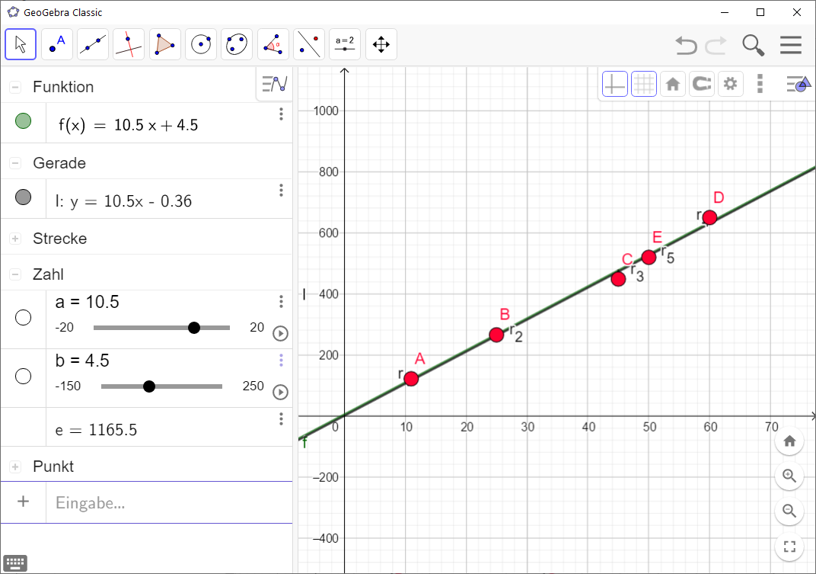
\includegraphics[height=0.75\textheight,keepaspectratio]{figures/ggb_lineare_regression.png}

\source{Prinzip Lineare Regression.ggb, \cite{seemann2024mlaz}}
\end{frame}

\begin{frame}{Sinn des Quadratischen Fehlers}
\begin{columns}
\column{0.01\textwidth}
\column{0.98\textwidth}

\centering
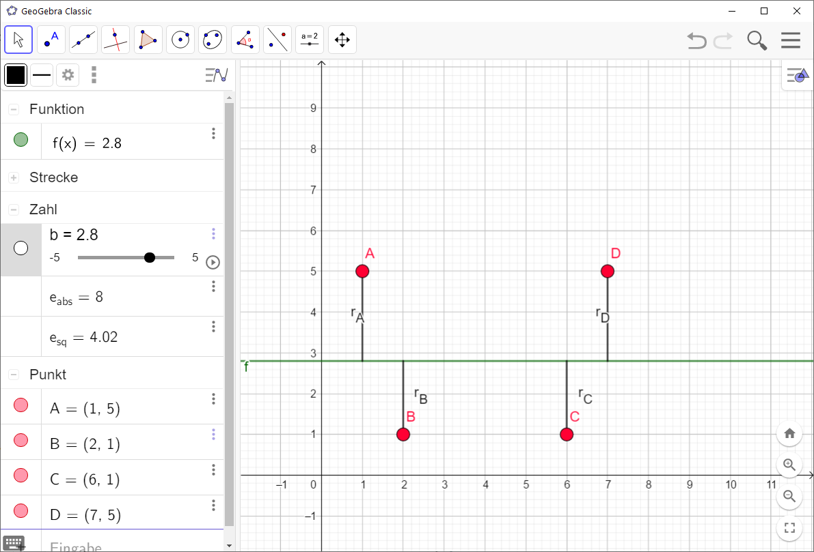
\includegraphics[height=0.75\textheight,keepaspectratio]{figures/ggb_quadratischer_fehler.png}

\end{columns}
\source{Prinzip Quadratischer Fehler.ggb, \cite{seemann2024mlaz}}
\end{frame}


\begin{frame}{Grundidee: Höhere Dimension}
\begin{columns}
\column{0.47\textwidth}
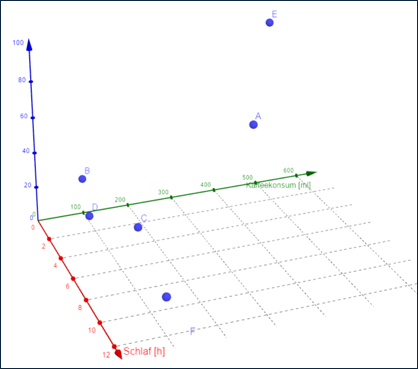
\includegraphics[height=0.7\textwidth,keepaspectratio]{figures/ggb_regession3D_A.png}
\column{0.48\textwidth}
\centering
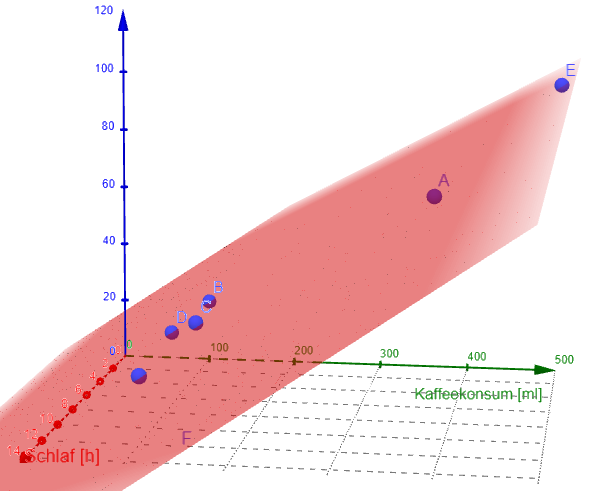
\includegraphics[height=0.7\textwidth,keepaspectratio]{figures/ggb_regession3D_B.png}
\end{columns}\par \medskip
Die lineare Regression funktioniert auch mit höherdimensionalen Eingangsräumen. In diesem Fall ist die lineare Funktion eine (Hyper)-Ebene.


\source{Lineare Regression 3D.ggb, \cite{seemann2024mlaz}}
\end{frame}


\begin{frame}{Umsetzung in Python}
\begin{columns}
\column{0.47\linewidth}
\centering
\includesvg[width=0.6\linewidth]{figures/jupyter_logo}

\column{0.6\linewidth}
\begin{itemize}
\item Jupyter Notebook ist Teil der Python-Distribution Anaconda
\item Startet einen lokalen Web-Server auf dem Rechner
\item Notebooks werden im Browser erstellt und bearbeitet
\item Unterstützung für interaktive Ausführung von Code und Visualisierungen
\item Auch in Visual Studio Code integrierbar und nutzbar
\end{itemize}
\end{columns}
\source{Bildquelle: \cite{jupyter_logo}}
\end{frame}


\begin{frame}[fragile]{Daten einlesen mit pandas}

\begin{columns}

\column{0.48\textwidth}

\textbf{pandas} ist eine zentrale Python-Bibliothek für die Datenanalyse.

\begin{itemize}
\item Einlesen strukturierter Daten (z.~B. CSV)
\item Zentrale Struktur: \texttt{DataFrame}
\item Filtern, Aggregieren, Transformieren
\item Standardwerkzeug in Data Science und KI
\end{itemize}

\column{0.48\textwidth}
\scriptsize
\begin{minted}[fontsize=\scriptsize]{python}
import pandas as pd

df = pd.read_csv("monatsmieten.csv")
\end{minted}

\vspace{0.5em}
\texttt{\textbf head()} zeigt die ersten fünf Einträge des Datensatzes an. So können wir uns ein erstes Bild von den Daten machen.
\begin{minted}[fontsize=\scriptsize]{python}
df.head()
\end{minted}
\raggedright
\begin{tabular}{rrr}
\textbf{} & \textbf{Quadratmeter} & \textbf{Kaltmiete} \\
0 & 70 & 771.45 \\
1 & 72 & 772.22 \\
2 & 91 & 1058.01 \\
3 & 58 & 650.30 \\
4 & 49 & 522.49 \\
\end{tabular}

\end{columns}
\source{\cite{seemann2024mlaz}, Datei: RegressionMieten.ipynb}
\end{frame}


\begin{frame}[fragile]{Darstellung der Daten}

\begin{columns}

\column{0.47\textwidth}
Die Bibliothek \textbf{matplotlib} ermöglicht die Visualisierung von Daten.

\medskip

Für uns besonders wichtig sind \textbf{Scatterplots}:

\begin{itemize}
\item eine Spalte als x-Werte
\item eine Spalte als y-Werte
\item zeigt Zusammenhänge zwischen Variablen
\end{itemize}

\medskip

Hier: Zusammenhang zwischen Wohnfläche und Miete

\column{0.48\textwidth}

\begin{minted}[fontsize=\scriptsize]{python}
%matplotlib inline # Grafik im Notebook
import matplotlib.pyplot as plt

plt.scatter(df["Quadratmeter"],
            df["Kaltmiete"])
plt.show()
\end{minted}
\includesvg[width=\linewidth]{figures/scatter_quadratmeter_miete}
\end{columns}
\source{\cite{seemann2024mlaz}, Datei: RegressionMieten.ipynb}
\note{das \texttt{plt.show()} braucht man nur außerhalb von Jupyter}
\end{frame}

\begin{frame}{Training eines Regressionsmodells}

\begin{columns}

\column{0.47\textwidth}
\textbf{Ziel:} Vorhersage des Preises anhand der Wohnungsgröße.
\begin{itemize}
\item Annähernd linearer Zusammenhang
\item Verwendung der \textbf{linearen Regression}
\end{itemize}

\medskip
\textbf{Wichtiger Schritt:}
\begin{itemize}
\item Daten werden immer aufgeteilt \textbf{Train--Test Split}
\item 
Typisch:
\begin{itemize}
\item 70--80\,\% Training
\item 20--30\,\% Test
\end{itemize}
\end{itemize}

\column{0.48\textwidth}

\textbf{Ablauf:}
\begin{itemize}
\item Modell wird nur mit Trainingsdaten trainiert
\item Testdaten bleiben zunächst unbekannt
\item Nur so kann man die Qualität des Modells später gut einschätzen
\end{itemize}

\medskip

\begin{block}{Grundregel}
Ein Modell wird immer mit Daten getestet, die es beim Training nicht gesehen hat!
\end{block}

\end{columns}
\source{\cite{seemann2024mlaz}}
\end{frame}

\begin{frame}{Training des Regressionsmodells mit sklearn}
\small
\begin{columns}

\column{0.47\textwidth}
Für Analyseaufgaben verwenden wir die Python-Bibliothek \textbf{scikit-learn (sklearn)}.

\begin{itemize}
\item Standardwerkzeug im Machine Learning
\item Einsatz auch im professionellen Umfeld
\item Viele Algorithmen und Hilfsfunktionen
\end{itemize}

Neben Lernverfahren bietet sklearn auch Werkzeuge zur \textbf{Datenvorbereitung}.

\column{0.48\textwidth}

\textbf{Wichtige Funktion:}
\begin{itemize}
\item \texttt{train\_test\_split}
\end{itemize}

\textbf{Aufgabe:}
\begin{itemize}
\item Aufteilung der Daten in Trainings- und Testmenge
\end{itemize}

\textbf{Vorteile:}
\begin{itemize}
\item automatisierter Train--Test Split
\item konsistente Vorbereitung der Daten
\item Grundlage für Bewertung des Modells
\end{itemize}

\end{columns}
\source{\cite{seemann2024mlaz}}
\end{frame}



\begin{frame}[fragile]{Python: Training des Regressionsmodells}
\medskip
Aufteilung in Trainings- und Testdaten:
\begin{minted}[fontsize=\scriptsize]{python}
from sklearn.model_selection import train_test_split
X = df[["Quadratmeter"]].to_numpy()  # pandas DataFrame -> NumPy Array
Y = df[["Kaltmiete"]].to_numpy()
X_train, X_test, Y_train, Y_test = train_test_split(X, Y, random_state=0)
\end{minted}

\begin{columns}
\column{0.47\textwidth}

Wir betrachten die Aufteilung im Scatterplot:

\begin{minted}[fontsize=\scriptsize]{python}
%matplotlib inline
import matplotlib.pyplot as plt

plt.scatter(X_train, Y_train)
plt.scatter(X_test, Y_test)
\end{minted}

\column{0.47\textwidth}
\includesvg[width=\linewidth]{figures/scatter_quadratmeter_miete_train_test}
\end{columns}
\source{\cite{seemann2024mlaz}, Datei: RegressionMieten.ipynb}
\end{frame}

\begin{frame}[fragile]{Python: Training des Regressionsmodells}

\begin{columns}

\column{0.35\textwidth}
\footnotesize
\textbf{Training des Modells:}
Das Regressionsmodell wird mit den Trainingsdaten angepasst.
\begin{itemize}
\item Wahl des Modelltyps: Lineare Regression
\item Anpassung an Trainingsdaten mit \texttt{fit()}
\item Bestimmung von Steigung und Achsenabschnitt
\end{itemize}

\medskip

\textbf{Ergebnis:}
\begin{itemize}
\item Funktion der Form: $y = a \cdot x + b$
\end{itemize}

\column{0.6\textwidth}

\begin{minted}[fontsize=\footnotesize]{python}
from sklearn.linear_model import LinearRegression

model = LinearRegression()
model.fit(X_train, Y_train)

print("Achsenabschnitt b:", model.intercept_)
print("Steigung a:", model.coef_)
\end{minted}
    \footnotesize
\begin{verbatim}
Achsenabschnitt b: [18.42935284]
Steigung a: [[10.72967643]]
\end{verbatim}

\end{columns}
\source{\cite{seemann2024mlaz}, Datei: RegressionMieten.ipynb}
\end{frame}


\begin{frame}[fragile]{Visualisierung der Regressionsgerade}

\begin{columns}

\column{0.35\textwidth}
\textbf{Idee:}
\begin{itemize}
\item Darstellung der Testdaten (rot)
\item Einzeichnen der gelernten Regressionsgeraden (blau)
\item Abstand zur Gerade = Vorhersagefehler
\end{itemize}

\column{0.60\textwidth}

\begin{minted}[fontsize=\footnotesize]{python}
plt.scatter(X_test, Y_test, color="red")
plt.plot(X_test, predicted, color="blue")
plt.show()
\end{minted}


\centering
\includesvg[width=0.7\linewidth]{figures/scatter_quadratmeter_regression}

\end{columns}
\source{\cite{seemann2024mlaz}, Datei: RegressionMieten.ipynb}
\end{frame}


\begin{frame}[fragile]{Vorhersagen treffen mit dem Modell}
\small
\begin{columns}

\column{0.47\textwidth}
\begin{itemize}
\item Das trainierte Modell kann neue Werte vorhersagen
\item Eingabe: neue, unbekannte Datenpunkte
\item Ausgabe: geschätzter Zielwert
\end{itemize}

\medskip
\textbf{Wichtig:}
\begin{itemize}
\item \texttt{predict()} arbeitet auf mehreren Datenpunkten gleichzeitig
\item Jeder Datenpunkt kann \textbf{mehrdimensional} sein
\item Daher immer Eingabe als Liste von Vektoren (Tensor)
\end{itemize}

\column{0.48\textwidth}

Wie hoch ist die Miete für eine Wohnung mit 120\,m\textsuperscript{2}?

\begin{minted}[fontsize=\small]{python}
rent = model.predict([[120]])
print(rent)
\end{minted}

\medskip

\textbf{Ausgabe:}

\texttt{[[1305.99052472]]}

\medskip

\textbf{Interpretation:}
\begin{itemize}
\item Modell sagt ca. 1306\,€ Miete voraus
\item Ergebnis ist ein Array (auch für mehrere Eingaben)
\end{itemize}

\end{columns}
\source{Datei: RegressionMieten.ipynb}
\end{frame}


\makequizpage{\QUIZURL}{\QUIZQRCODE}{\QUIZIMAGE}


\begin{frame}{Übung: Multiple Regression mit Auto-Daten}
\begin{columns}

\column{0.65\textwidth}
\footnotesize
Die Datei \texttt{auto-mpg.csv} enthält Daten zum Kraftstoffverbrauch in den USA.

\textbf{Aufgaben:}
\begin{itemize}
\item Analysieren Sie den Zusammenhang zwischen dem Fahrzeuggewicht (\texttt{weight})
und dem Verbrauch in mpg (\texttt{mpg})

\item Gehen Sie von einem annähernd linearen Zusammenhang aus

\item Trainieren Sie ein Regressionsmodell zur Vorhersage von \texttt{mpg}

\item Bestimmen Sie den erwarteten mpg-Wert für ein Fahrzeug mit 4000\,Pfund
\end{itemize}

\textbf{Hinweis:}
\begin{itemize}
\item $1\,\text{l/100km} = 235.21\,\text{mpg}$
\item Teilen Sie 235.21 durch den mpg-Wert, dann haben Sie den Verbrauch in Litern pro 100 km.
\end{itemize}

\column{0.3\textwidth}

\twemoji[width=0.9\linewidth]{laptop}

\end{columns}
\source{Lösung: Regression-mpg.ipynb}
\end{frame}

\makequestionspage{\FRAGENIMAGE}

%%%%%%%%%%%%%%%%%%%%%%%%%%%%%%%%%%%%%%%%%%%%%%%%%%%%%%%%%%%%%%%%%%%
\begin{frame}{Wie funktioniert jetzt das Training genau?}

\begin{columns}

\column{0.47\textwidth}

Die lineare Regression wählt die \textbf{am besten passenden Parameter} für die lineare Regressionsfunktion mithilfe der \textbf{Methode der kleinsten Quadrate}.

\medskip

\textbf{Grundproblem:}
\begin{itemize}
\item Wir haben eine Menge $D \subseteq \mathbb{R}^n \times \mathbb{R}$ von Datenpunkten.
\item Jeder Datenpunkt hat die Form $((x_1, \dots, x_n), y)$.
\item Wir suchen eine Funktion $f: \mathbb{R}^n \to \mathbb{R}$, deren Graph möglichst nah an den Datenpunkten liegt.
\end{itemize}

\column{0.48\textwidth}
\includesvg[width=\linewidth]{figures/pruefungsleistung_regression}
\end{columns}

\source{\cite{Frochte2020}}
\end{frame}






\begin{frame}{Lineare Modelle und Hyperebenen}
\footnotesize
\begin{columns}

\column{0.47\textwidth}
Bei einem \textbf{linearen Modell} mit $n$-dimensionalem Eingangsraum hat die anpassbare Funktion $f: \mathbb{R}^n \to \mathbb{R}$ die Form
\[
    f(\mathbf{x} ) = u_0 + u_1\cdot x_1 + \dots + u_n \cdot x_n
\]
mit $u_0, \dots , u_n \in \mathbb{R}^n$. \medskip

Man schreibt das typischerweise als Skalarprodukt
\[
    f(\mathbf{x} ) = u_0 + \mathbf{b}^T \cdot \mathbf{x}  
\]
mit  $u_0\in \mathbb{R}, \mathbf{b}^T = (u_1, \dots, u_n) \in \mathbb{R}^n$. 


\column{0.47\textwidth}
\begin{block}{\footnotesize Ebenengleichung}
Aus der Schule kennen Sie die Darstellung bereits als \textbf{Koordinatenform} einer Ebene. Man im  2D-Eingangsraum schreibt man
\[
z=ax+ay+c
\]
\end{block}

\begin{blockC3}{\footnotesize Hyperebenen}
Lineare Modelle beschreiben im 2D-Eingangsraum \textbf{Ebenen}, im 1D-Eingangsraum \textbf{Geraden} und für allgemeine Eingangsräume \textbf{Hyperebeben}
\end{blockC3}

\end{columns}

\source{\cite{Frochte2020}}

\note{Die Wahl der Parameter bestimmt die konkrete Lage der Ebene}

\end{frame}

%%%%%%%%%%%%%%%%%%%%%%%%%%%%%%%%%%%%%%%%%%%%%%%%%%%%%%%%%%%%%%%%
\begin{frame}{Beispiel: Boston Housing Dataset}


    
    \begin{columns}
\column{0.35\textwidth}

Wir berechnen ein Regressionsmodell für den \textbf{Boston Housing Dataset}.

\textbf{Aufgabe:}
\begin{itemize}
\item 13 Eingangsmerkmale
\item $\rightarrow$ Vorhersage des Medianpreises
\end{itemize}
\centering
\twemoji[width=0.5\linewidth]{houses}

\column{0.60\textwidth}
\textbf{Merkmale (Auszug):}
\begin{itemize}
\item Kriminalitätsrate pro Kopf
\item Anteil Wohnbauland ($> 25{,}000$ sq ft)
\item Anteil Gewerbeflächen (nicht Einzelhandel)
\item Stickoxidkonzentration
\item Anteil alter Gebäude (vor 1940)
\item Entfernung zu Arbeitszentren
\item Zugang zu Autobahnen
\item Schüler--Lehrer-Verhältnis
\item Anteil sozial benachteiligter Bevölkerung
\item Medianpreis von Häusern (in 1000 \$)
\end{itemize}
\end{columns}
\source{\cite{Frochte2020}}
\end{frame}

\begin{frame}[fragile]{Boston Housing Dataset in Python}

Wir betrachten den Datensatz mit pandas:

\begin{minted}[fontsize=\small]{python}
import pandas as pd

df = pd.read_csv("BostonHousing.csv")
df.head()
\end{minted}

\medskip

\textbf{Ausgabe:}
{
\tiny
\begin{tabular}{rcccccccccccccc}
\textbf{} & \textbf{CRIM} & \textbf{ZN} & \textbf{INDUS} & \textbf{CHAS} & \textbf{NOX} & \textbf{RM} & \textbf{AGE} & \textbf{DIS} & \textbf{RAD} & \textbf{TAX} & \textbf{PTRATIO} & \textbf{LSTAT} & \textbf{MEDV} & \textbf{CAT. MEDV} \\
0 & 0.00632 & 18.0 & 2.31 & 0 & 0.538 & 6.575 & 65.2 & 4.0900 & 1 & 296 & 15.3 & 4.98 & 24.0 & 0 \\
1 & 0.02731 & 0.0 & 7.07 & 0 & 0.469 & 6.421 & 78.9 & 4.9671 & 2 & 242 & 17.8 & 9.14 & 21.6 & 0 \\
2 & 0.02729 & 0.0 & 7.07 & 0 & 0.469 & 7.185 & 61.1 & 4.9671 & 2 & 242 & 17.8 & 4.03 & 34.7 & 1 \\
3 & 0.03237 & 0.0 & 2.18 & 0 & 0.458 & 6.998 & 45.8 & 6.0622 & 3 & 222 & 18.7 & 2.94 & 33.4 & 1 \\
4 & 0.06905 & 0.0 & 2.18 & 0 & 0.458 & 7.147 & 54.2 & 6.0622 & 3 & 222 & 18.7 & 5.33 & 36.2 & 1 \\
\end{tabular}
} \par \bigskip
\textbf{MEDV} ist unsere Zielgröße. Die anderen 13 Werte bilden unseren Merkmalsraum $X\subseteq\mathbb{R}^{13}$.

\end{frame}


\makequizpage{\QUIZURL}{\QUIZQRCODE}{\QUIZIMAGE}
\makequestionspage{\FRAGENIMAGE}